\documentclass{standalone}
\usepackage{tikz}
\usepackage{ctex,siunitx}
\setCJKmainfont{Noto Serif CJK SC}
\usepackage{tkz-euclide}
\usepackage{amsmath}
\usetikzlibrary{patterns, calc,3d}
\usetikzlibrary {decorations.pathmorphing,decorations.pathreplacing,decorations.shapes}
\begin{document}
\small
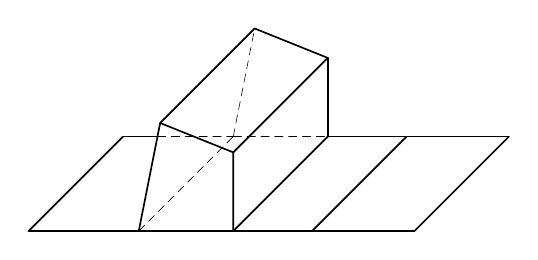
\begin{tikzpicture}[>=latex,scale=1.0]
  \tkzDefPoints{0/0/A,1.2/0/B,1.2/1/C,2.2/0/E,3.5/0/F,-1.4/0/G,-0.2/1.2/G'}
  \tkzInterCC(A,G)(C,B)\tkzGetPoints{D}{O}
  \tkzDefPointsBy[translation=from G to G'](A,B,C,D,E,F){A',B',C',D',E',F'}
  \tkzInterLL(G',A')(A,D)\tkzGetPoint{M}
  \tkzDrawPolygon[semithick](A,B,C,D)
  \tkzDrawSegments[semithick](B,B' C,C' D,D' E,E' F,F' G,G' G,F B',C' C',D' B',F' G',M)
  \tkzDrawSegments[densely dashed](A,A' A',B' A',D' M,A')
  % \tkzLabelPoints(A,B,C)
  % \tkzLabelPoints[above left](F,E,D)
  % \tkzLabelPoints[left](F',E')
  % \tkzLabelPoints[right](A',B',C',D')
\end{tikzpicture}
\end{document}